\documentclass{standalone}
\usepackage{tikz}
\usetikzlibrary{patterns}
\usetikzlibrary{positioning}
\usetikzlibrary{patterns, positioning}
\usetikzlibrary{shapes.misc}
\usepackage[outline]{contour}
\contourlength{1.5pt} 
\usetikzlibrary{calc}
        \usepackage{relsize}
        \tikzset{fontscale/.style = {font=\relsize{#1}}}

\begin{document}
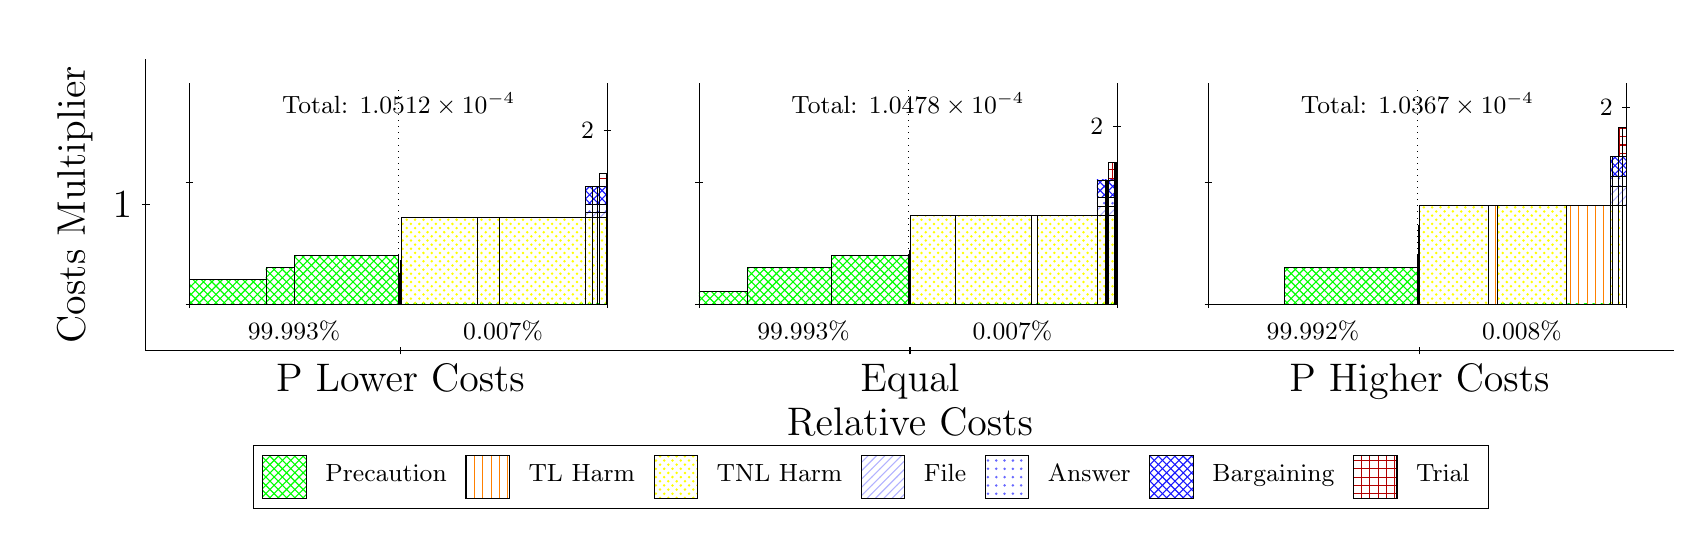
\begin{tikzpicture}
\clip(-0.5,-1.1) rectangle +(20.91,6.2);
\draw[black] (1,1) -- (1,4.7);
\node[rotate=90, fontscale=2, anchor=center] at (0.1, 2.85) {Costs Multiplier};
\draw[black] (0.95,2.85) -- (1.05,2.85);
\node[fontscale=2, anchor=east] at (0.95, 2.85) {1};

\draw[black] (1,1) -- (20.41,1);
\node[fontscale=2, anchor=center] at (10.705, 0.1) {Relative Costs};
\draw[black] (4.235,0.95) -- (4.235,1.05);
\node[fontscale=2, anchor=north] at (4.235, 0.95) {P Lower Costs};
\draw[black] (10.705,0.95) -- (10.705,1.05);
\node[fontscale=2, anchor=north] at (10.705, 0.95) {Equal};
\draw[black] (17.175,0.95) -- (17.175,1.05);
\node[fontscale=2, anchor=north] at (17.175, 0.95) {P Higher Costs};


\draw[pattern=crosshatch, pattern color=green,draw=black,very thin] (1.5556,1.592) rectangle (2.5248,1.9012);
\draw[pattern=crosshatch, pattern color=green,draw=black,very thin] (2.5248,1.592) rectangle (2.8828,2.0557);
\draw[pattern=crosshatch, pattern color=green,draw=black,very thin] (2.8828,1.592) rectangle (4.21,2.2103);
\draw[pattern=crosshatch, pattern color=green,draw=black,very thin] (4.21,1.592) rectangle (4.2203,1.592);
\draw[pattern=north east lines, pattern color=blue!30,draw=black,very thin] (4.21,1.592) rectangle (4.2203,1.6471);
\draw[pattern=dots,  pattern color=blue!60,draw=black,very thin] (4.21,1.6471) rectangle (4.2203,1.7573);
\draw[pattern=crosshatch,      pattern color=blue!90,draw=black,very thin] (4.21,1.7573) rectangle (4.2203,1.9778);
\draw[pattern=crosshatch, pattern color=green,draw=black,very thin] (4.2203,1.592) rectangle (4.2328,1.592);
\draw[pattern=north east lines, pattern color=blue!30,draw=black,very thin] (4.2203,1.592) rectangle (4.2328,1.6471);
\draw[pattern=dots,  pattern color=blue!60,draw=black,very thin] (4.2203,1.6471) rectangle (4.2328,1.7573);
\draw[pattern=crosshatch,      pattern color=blue!90,draw=black,very thin] (4.2203,1.7573) rectangle (4.2328,1.9778);
\draw[pattern=crosshatch, pattern color=green,draw=black,very thin] (4.2328,1.592) rectangle (4.2462,1.592);
\draw[pattern=north east lines, pattern color=blue!30,draw=black,very thin] (4.2328,1.592) rectangle (4.2462,1.6471);
\draw[pattern=dots,  pattern color=blue!60,draw=black,very thin] (4.2328,1.6471) rectangle (4.2462,1.7573);
\draw[pattern=crosshatch,      pattern color=blue!90,draw=black,very thin] (4.2328,1.7573) rectangle (4.2462,1.9778);
\draw[pattern=grid,            pattern color=red!70!black,draw=black,very thin] (4.2328,1.9778) rectangle (4.2462,2.1431);
\draw[pattern=crosshatch, pattern color=green,draw=black,very thin] (4.2462,1.592) rectangle (5.2058,1.592);
\draw[pattern=crosshatch dots, pattern color=yellow,draw=black,very thin] (4.2462,1.592) rectangle (5.2058,2.6941);
\draw[pattern=crosshatch, pattern color=green,draw=black,very thin] (5.2058,1.592) rectangle (5.2096,1.592);
\draw[pattern=vertical lines, pattern color=orange,draw=black,very thin] (5.2058,1.592) rectangle (5.2096,2.6941);
\draw[pattern=crosshatch, pattern color=green,draw=black,very thin] (5.2096,1.592) rectangle (5.4901,1.592);
\draw[pattern=crosshatch dots, pattern color=yellow,draw=black,very thin] (5.2096,1.592) rectangle (5.4901,2.6941);
\draw[pattern=crosshatch, pattern color=green,draw=black,very thin] (5.4901,1.592) rectangle (5.4939,1.592);
\draw[pattern=vertical lines, pattern color=orange,draw=black,very thin] (5.4901,1.592) rectangle (5.4939,2.6941);
\draw[pattern=crosshatch, pattern color=green,draw=black,very thin] (5.4939,1.592) rectangle (6.5852,1.592);
\draw[pattern=crosshatch dots, pattern color=yellow,draw=black,very thin] (5.4939,1.592) rectangle (6.5852,2.6941);
\draw[pattern=crosshatch, pattern color=green,draw=black,very thin] (6.5852,1.592) rectangle (6.6641,1.592);
\draw[pattern=crosshatch dots, pattern color=yellow,draw=black,very thin] (6.5852,1.592) rectangle (6.6641,2.6941);
\draw[pattern=north east lines, pattern color=blue!30,draw=black,very thin] (6.5852,2.6941) rectangle (6.6641,2.7492);
\draw[pattern=dots,  pattern color=blue!60,draw=black,very thin] (6.5852,2.7492) rectangle (6.6641,2.8594);
\draw[pattern=crosshatch,      pattern color=blue!90,draw=black,very thin] (6.5852,2.8594) rectangle (6.6641,3.0799);
\draw[pattern=crosshatch, pattern color=green,draw=black,very thin] (6.6641,1.592) rectangle (6.6695,1.592);
\draw[pattern=vertical lines, pattern color=orange,draw=black,very thin] (6.6641,1.592) rectangle (6.6695,2.6941);
\draw[pattern=north east lines, pattern color=blue!30,draw=black,very thin] (6.6641,2.6941) rectangle (6.6695,2.7492);
\draw[pattern=dots,  pattern color=blue!60,draw=black,very thin] (6.6641,2.7492) rectangle (6.6695,2.8594);
\draw[pattern=crosshatch,      pattern color=blue!90,draw=black,very thin] (6.6641,2.8594) rectangle (6.6695,3.0799);
\draw[pattern=crosshatch, pattern color=green,draw=black,very thin] (6.6695,1.592) rectangle (6.7357,1.592);
\draw[pattern=crosshatch dots, pattern color=yellow,draw=black,very thin] (6.6695,1.592) rectangle (6.7357,2.6941);
\draw[pattern=north east lines, pattern color=blue!30,draw=black,very thin] (6.6695,2.6941) rectangle (6.7357,2.7492);
\draw[pattern=dots,  pattern color=blue!60,draw=black,very thin] (6.6695,2.7492) rectangle (6.7357,2.8594);
\draw[pattern=crosshatch,      pattern color=blue!90,draw=black,very thin] (6.6695,2.8594) rectangle (6.7357,3.0799);
\draw[pattern=crosshatch, pattern color=green,draw=black,very thin] (6.7357,1.592) rectangle (6.7561,1.592);
\draw[pattern=vertical lines, pattern color=orange,draw=black,very thin] (6.7357,1.592) rectangle (6.7561,2.6941);
\draw[pattern=north east lines, pattern color=blue!30,draw=black,very thin] (6.7357,2.6941) rectangle (6.7561,2.7492);
\draw[pattern=dots,  pattern color=blue!60,draw=black,very thin] (6.7357,2.7492) rectangle (6.7561,2.8594);
\draw[pattern=crosshatch,      pattern color=blue!90,draw=black,very thin] (6.7357,2.8594) rectangle (6.7561,3.0799);
\draw[pattern=crosshatch, pattern color=green,draw=black,very thin] (6.7561,1.592) rectangle (6.8439,1.592);
\draw[pattern=crosshatch dots, pattern color=yellow,draw=black,very thin] (6.7561,1.592) rectangle (6.8439,2.6941);
\draw[pattern=north east lines, pattern color=blue!30,draw=black,very thin] (6.7561,2.6941) rectangle (6.8439,2.7492);
\draw[pattern=dots,  pattern color=blue!60,draw=black,very thin] (6.7561,2.7492) rectangle (6.8439,2.8594);
\draw[pattern=crosshatch,      pattern color=blue!90,draw=black,very thin] (6.7561,2.8594) rectangle (6.8439,3.0799);
\draw[pattern=grid,            pattern color=red!70!black,draw=black,very thin] (6.7561,3.0799) rectangle (6.8439,3.2452);
\draw[pattern=crosshatch, pattern color=green,draw=black,very thin] (6.8439,1.592) rectangle (6.8644,1.592);
\draw[pattern=vertical lines, pattern color=orange,draw=black,very thin] (6.8439,1.592) rectangle (6.8644,2.6941);
\draw[pattern=north east lines, pattern color=blue!30,draw=black,very thin] (6.8439,2.6941) rectangle (6.8644,2.7492);
\draw[pattern=dots,  pattern color=blue!60,draw=black,very thin] (6.8439,2.7492) rectangle (6.8644,2.8594);
\draw[pattern=crosshatch,      pattern color=blue!90,draw=black,very thin] (6.8439,2.8594) rectangle (6.8644,3.0799);
\draw[pattern=grid,            pattern color=red!70!black,draw=black,very thin] (6.8439,3.0799) rectangle (6.8644,3.2452);
\node[font=\small,text=black,anchor=north] at (4.21, 4.4) {Total: $1.0512\times 10^{-4}$};
\draw[black,very thin] (1.5556,1.592) -- (1.5556,4.4);
\draw[black,very thin] (1.5056,1.592) -- (1.6056,1.592);
\node[font=\small,text=black, anchor=west] at (1.5056, 1.592) {};
\draw[black,very thin] (1.5056,3.1378) -- (1.6056,3.1378);
\node[font=\small,text=black, anchor=west] at (1.5056, 3.1378) {};

\draw[black,dotted,very thin] (4.21,1.6762) -- (4.21,4.3158);
\draw[black,very thin] (6.8644,1.592) -- (6.8644,4.4);
\draw[black,very thin] (6.8144,3.7962) -- (6.9144,3.7962);
\node[font=\small,text=black, anchor=east] at (6.8144, 3.7962) {\contour{white}{2}};

\draw[black,very thin] (1.5556,1.592) -- (6.8644,1.592);
\draw[black,very thin] (1.5556,1.542) -- (1.5556,1.642);
\node[font=\small,text=black, anchor=north] at (1.5556, 1.542) {};
\draw[black,very thin] (6.8644,1.542) -- (6.8644,1.642);
\node[font=\small,text=black, anchor=north] at (6.8644, 1.542) {};

\node[font=\small,text=black,anchor=south] at (2.8828, 0.992) {99.993\%};
\node[font=\small,text=black,anchor=south] at (5.5372, 0.992) {0.007\%};

\draw[pattern=crosshatch, pattern color=green,draw=black,very thin] (8.0256,1.592) rectangle (8.6361,1.7466);
\draw[pattern=crosshatch, pattern color=green,draw=black,very thin] (8.6361,1.592) rectangle (9.7108,2.0557);
\draw[pattern=crosshatch, pattern color=green,draw=black,very thin] (9.7108,1.592) rectangle (10.68,2.2103);
\draw[pattern=crosshatch, pattern color=green,draw=black,very thin] (10.68,1.592) rectangle (10.693,1.592);
\draw[pattern=north east lines, pattern color=blue!30,draw=black,very thin] (10.68,1.592) rectangle (10.693,1.7045);
\draw[pattern=dots,  pattern color=blue!60,draw=black,very thin] (10.68,1.7045) rectangle (10.693,1.817);
\draw[pattern=crosshatch,      pattern color=blue!90,draw=black,very thin] (10.68,1.817) rectangle (10.693,2.0421);
\draw[pattern=crosshatch, pattern color=green,draw=black,very thin] (10.693,1.592) rectangle (10.698,1.592);
\draw[pattern=north east lines, pattern color=blue!30,draw=black,very thin] (10.693,1.592) rectangle (10.698,1.7046);
\draw[pattern=dots,  pattern color=blue!60,draw=black,very thin] (10.693,1.7046) rectangle (10.698,1.8171);
\draw[pattern=crosshatch,      pattern color=blue!90,draw=black,very thin] (10.693,1.8171) rectangle (10.698,2.0421);
\draw[pattern=crosshatch, pattern color=green,draw=black,very thin] (10.698,1.592) rectangle (10.707,1.592);
\draw[pattern=north east lines, pattern color=blue!30,draw=black,very thin] (10.698,1.592) rectangle (10.707,1.7045);
\draw[pattern=dots,  pattern color=blue!60,draw=black,very thin] (10.698,1.7045) rectangle (10.707,1.817);
\draw[pattern=crosshatch,      pattern color=blue!90,draw=black,very thin] (10.698,1.817) rectangle (10.707,2.0421);
\draw[pattern=grid,            pattern color=red!70!black,draw=black,very thin] (10.698,2.0421) rectangle (10.707,2.2671);
\draw[pattern=crosshatch, pattern color=green,draw=black,very thin] (10.707,1.592) rectangle (10.71,1.592);
\draw[pattern=north east lines, pattern color=blue!30,draw=black,very thin] (10.707,1.592) rectangle (10.71,1.7046);
\draw[pattern=dots,  pattern color=blue!60,draw=black,very thin] (10.707,1.7046) rectangle (10.71,1.8171);
\draw[pattern=crosshatch,      pattern color=blue!90,draw=black,very thin] (10.707,1.8171) rectangle (10.71,2.0421);
\draw[pattern=grid,            pattern color=red!70!black,draw=black,very thin] (10.707,2.0421) rectangle (10.71,2.2671);
\draw[pattern=crosshatch, pattern color=green,draw=black,very thin] (10.71,1.592) rectangle (11.28,1.592);
\draw[pattern=crosshatch dots, pattern color=yellow,draw=black,very thin] (10.71,1.592) rectangle (11.28,2.7172);
\draw[pattern=crosshatch, pattern color=green,draw=black,very thin] (11.28,1.592) rectangle (11.283,1.592);
\draw[pattern=vertical lines, pattern color=orange,draw=black,very thin] (11.28,1.592) rectangle (11.283,2.7172);
\draw[pattern=crosshatch, pattern color=green,draw=black,very thin] (11.283,1.592) rectangle (12.251,1.592);
\draw[pattern=crosshatch dots, pattern color=yellow,draw=black,very thin] (11.283,1.592) rectangle (12.251,2.7172);
\draw[pattern=crosshatch, pattern color=green,draw=black,very thin] (12.251,1.592) rectangle (12.321,1.592);
\draw[pattern=vertical lines, pattern color=orange,draw=black,very thin] (12.251,1.592) rectangle (12.321,2.7172);
\draw[pattern=crosshatch, pattern color=green,draw=black,very thin] (12.321,1.592) rectangle (13.08,1.592);
\draw[pattern=crosshatch dots, pattern color=yellow,draw=black,very thin] (12.321,1.592) rectangle (13.08,2.7172);
\draw[pattern=crosshatch, pattern color=green,draw=black,very thin] (13.08,1.592) rectangle (13.183,1.592);
\draw[pattern=crosshatch dots, pattern color=yellow,draw=black,very thin] (13.08,1.592) rectangle (13.183,2.7172);
\draw[pattern=north east lines, pattern color=blue!30,draw=black,very thin] (13.08,2.7172) rectangle (13.183,2.8297);
\draw[pattern=dots,  pattern color=blue!60,draw=black,very thin] (13.08,2.8297) rectangle (13.183,2.9422);
\draw[pattern=crosshatch,      pattern color=blue!90,draw=black,very thin] (13.08,2.9422) rectangle (13.183,3.1672);
\draw[pattern=crosshatch, pattern color=green,draw=black,very thin] (13.183,1.592) rectangle (13.198,1.592);
\draw[pattern=vertical lines, pattern color=orange,draw=black,very thin] (13.183,1.592) rectangle (13.198,2.7172);
\draw[pattern=north east lines, pattern color=blue!30,draw=black,very thin] (13.183,2.7172) rectangle (13.198,2.8297);
\draw[pattern=dots,  pattern color=blue!60,draw=black,very thin] (13.183,2.8297) rectangle (13.198,2.9422);
\draw[pattern=crosshatch,      pattern color=blue!90,draw=black,very thin] (13.183,2.9422) rectangle (13.198,3.1672);
\draw[pattern=crosshatch, pattern color=green,draw=black,very thin] (13.198,1.592) rectangle (13.208,1.592);
\draw[pattern=crosshatch dots, pattern color=yellow,draw=black,very thin] (13.198,1.592) rectangle (13.208,2.7172);
\draw[pattern=north east lines, pattern color=blue!30,draw=black,very thin] (13.198,2.7172) rectangle (13.208,2.8297);
\draw[pattern=dots,  pattern color=blue!60,draw=black,very thin] (13.198,2.8297) rectangle (13.208,2.9422);
\draw[pattern=crosshatch,      pattern color=blue!90,draw=black,very thin] (13.198,2.9422) rectangle (13.208,3.1673);
\draw[pattern=crosshatch, pattern color=green,draw=black,very thin] (13.208,1.592) rectangle (13.228,1.592);
\draw[pattern=vertical lines, pattern color=orange,draw=black,very thin] (13.208,1.592) rectangle (13.228,2.7172);
\draw[pattern=north east lines, pattern color=blue!30,draw=black,very thin] (13.208,2.7172) rectangle (13.228,2.8297);
\draw[pattern=dots,  pattern color=blue!60,draw=black,very thin] (13.208,2.8297) rectangle (13.228,2.9422);
\draw[pattern=crosshatch,      pattern color=blue!90,draw=black,very thin] (13.208,2.9422) rectangle (13.228,3.1673);
\draw[pattern=crosshatch, pattern color=green,draw=black,very thin] (13.228,1.592) rectangle (13.303,1.592);
\draw[pattern=crosshatch dots, pattern color=yellow,draw=black,very thin] (13.228,1.592) rectangle (13.303,2.7172);
\draw[pattern=north east lines, pattern color=blue!30,draw=black,very thin] (13.228,2.7172) rectangle (13.303,2.8297);
\draw[pattern=dots,  pattern color=blue!60,draw=black,very thin] (13.228,2.8297) rectangle (13.303,2.9422);
\draw[pattern=crosshatch,      pattern color=blue!90,draw=black,very thin] (13.228,2.9422) rectangle (13.303,3.1672);
\draw[pattern=grid,            pattern color=red!70!black,draw=black,very thin] (13.228,3.1672) rectangle (13.303,3.3923);
\draw[pattern=crosshatch, pattern color=green,draw=black,very thin] (13.303,1.592) rectangle (13.314,1.592);
\draw[pattern=vertical lines, pattern color=orange,draw=black,very thin] (13.303,1.592) rectangle (13.314,2.7172);
\draw[pattern=north east lines, pattern color=blue!30,draw=black,very thin] (13.303,2.7172) rectangle (13.314,2.8297);
\draw[pattern=dots,  pattern color=blue!60,draw=black,very thin] (13.303,2.8297) rectangle (13.314,2.9422);
\draw[pattern=crosshatch,      pattern color=blue!90,draw=black,very thin] (13.303,2.9422) rectangle (13.314,3.1672);
\draw[pattern=grid,            pattern color=red!70!black,draw=black,very thin] (13.303,3.1672) rectangle (13.314,3.3923);
\draw[pattern=crosshatch, pattern color=green,draw=black,very thin] (13.314,1.592) rectangle (13.326,1.592);
\draw[pattern=crosshatch dots, pattern color=yellow,draw=black,very thin] (13.314,1.592) rectangle (13.326,2.7172);
\draw[pattern=north east lines, pattern color=blue!30,draw=black,very thin] (13.314,2.7172) rectangle (13.326,2.8297);
\draw[pattern=dots,  pattern color=blue!60,draw=black,very thin] (13.314,2.8297) rectangle (13.326,2.9422);
\draw[pattern=crosshatch,      pattern color=blue!90,draw=black,very thin] (13.314,2.9422) rectangle (13.326,3.1673);
\draw[pattern=grid,            pattern color=red!70!black,draw=black,very thin] (13.314,3.1673) rectangle (13.326,3.3923);
\draw[pattern=crosshatch, pattern color=green,draw=black,very thin] (13.326,1.592) rectangle (13.334,1.592);
\draw[pattern=vertical lines, pattern color=orange,draw=black,very thin] (13.326,1.592) rectangle (13.334,2.7172);
\draw[pattern=north east lines, pattern color=blue!30,draw=black,very thin] (13.326,2.7172) rectangle (13.334,2.8297);
\draw[pattern=dots,  pattern color=blue!60,draw=black,very thin] (13.326,2.8297) rectangle (13.334,2.9422);
\draw[pattern=crosshatch,      pattern color=blue!90,draw=black,very thin] (13.326,2.9422) rectangle (13.334,3.1673);
\draw[pattern=grid,            pattern color=red!70!black,draw=black,very thin] (13.326,3.1673) rectangle (13.334,3.3923);
\node[font=\small,text=black,anchor=north] at (10.68, 4.4) {Total: $1.0478\times 10^{-4}$};
\draw[black,very thin] (8.0256,1.592) -- (8.0256,4.4);
\draw[black,very thin] (7.9756,1.592) -- (8.0756,1.592);
\node[font=\small,text=black, anchor=west] at (7.9756, 1.592) {};
\draw[black,very thin] (7.9756,3.1378) -- (8.0756,3.1378);
\node[font=\small,text=black, anchor=west] at (7.9756, 3.1378) {};

\draw[black,dotted,very thin] (10.68,1.6762) -- (10.68,4.3158);
\draw[black,very thin] (13.334,1.592) -- (13.334,4.4);
\draw[black,very thin] (13.284,3.8423) -- (13.384,3.8423);
\node[font=\small,text=black, anchor=east] at (13.284, 3.8423) {\contour{white}{2}};

\draw[black,very thin] (8.0256,1.592) -- (13.334,1.592);
\draw[black,very thin] (8.0256,1.542) -- (8.0256,1.642);
\node[font=\small,text=black, anchor=north] at (8.0256, 1.542) {};
\draw[black,very thin] (13.334,1.542) -- (13.334,1.642);
\node[font=\small,text=black, anchor=north] at (13.334, 1.542) {};

\node[font=\small,text=black,anchor=south] at (9.3528, 0.992) {99.993\%};
\node[font=\small,text=black,anchor=south] at (12.007, 0.992) {0.007\%};

\draw[pattern=crosshatch, pattern color=green,draw=black,very thin] (15.465,1.592) rectangle (17.15,2.0557);
\draw[pattern=north east lines, pattern color=blue!30,draw=black,very thin] (17.15,1.592) rectangle (17.161,1.8416);
\draw[pattern=dots,  pattern color=blue!60,draw=black,very thin] (17.15,1.8416) rectangle (17.161,1.9664);
\draw[pattern=crosshatch,      pattern color=blue!90,draw=black,very thin] (17.15,1.9664) rectangle (17.161,2.216);
\draw[pattern=north east lines, pattern color=blue!30,draw=black,very thin] (17.161,1.592) rectangle (17.171,1.8416);
\draw[pattern=dots,  pattern color=blue!60,draw=black,very thin] (17.161,1.8416) rectangle (17.171,1.9664);
\draw[pattern=crosshatch,      pattern color=blue!90,draw=black,very thin] (17.161,1.9664) rectangle (17.171,2.216);
\draw[pattern=grid,            pattern color=red!70!black,draw=black,very thin] (17.161,2.216) rectangle (17.171,2.5904);
\draw[pattern=crosshatch dots, pattern color=yellow,draw=black,very thin] (17.171,1.592) rectangle (18.048,2.84);
\draw[pattern=vertical lines, pattern color=orange,draw=black,very thin] (18.048,1.592) rectangle (18.163,2.84);
\draw[pattern=crosshatch, pattern color=green,draw=black,very thin] (18.163,1.592) rectangle (19.034,1.592);
\draw[pattern=crosshatch dots, pattern color=yellow,draw=black,very thin] (18.163,1.592) rectangle (19.034,2.84);
\draw[pattern=crosshatch, pattern color=green,draw=black,very thin] (19.034,1.592) rectangle (19.596,1.592);
\draw[pattern=vertical lines, pattern color=orange,draw=black,very thin] (19.034,1.592) rectangle (19.596,2.84);
\draw[pattern=crosshatch dots, pattern color=yellow,draw=black,very thin] (19.596,1.592) rectangle (19.624,2.84);
\draw[pattern=north east lines, pattern color=blue!30,draw=black,very thin] (19.596,2.84) rectangle (19.624,3.0896);
\draw[pattern=dots,  pattern color=blue!60,draw=black,very thin] (19.596,3.0896) rectangle (19.624,3.2144);
\draw[pattern=crosshatch,      pattern color=blue!90,draw=black,very thin] (19.596,3.2144) rectangle (19.624,3.464);
\draw[pattern=vertical lines, pattern color=orange,draw=black,very thin] (19.624,1.592) rectangle (19.702,2.84);
\draw[pattern=north east lines, pattern color=blue!30,draw=black,very thin] (19.624,2.84) rectangle (19.702,3.0896);
\draw[pattern=dots,  pattern color=blue!60,draw=black,very thin] (19.624,3.0896) rectangle (19.702,3.2144);
\draw[pattern=crosshatch,      pattern color=blue!90,draw=black,very thin] (19.624,3.2144) rectangle (19.702,3.464);
\draw[pattern=crosshatch dots, pattern color=yellow,draw=black,very thin] (19.702,1.592) rectangle (19.751,2.84);
\draw[pattern=north east lines, pattern color=blue!30,draw=black,very thin] (19.702,2.84) rectangle (19.751,3.0896);
\draw[pattern=dots,  pattern color=blue!60,draw=black,very thin] (19.702,3.0896) rectangle (19.751,3.2144);
\draw[pattern=crosshatch,      pattern color=blue!90,draw=black,very thin] (19.702,3.2144) rectangle (19.751,3.464);
\draw[pattern=grid,            pattern color=red!70!black,draw=black,very thin] (19.702,3.464) rectangle (19.751,3.8384);
\draw[pattern=vertical lines, pattern color=orange,draw=black,very thin] (19.751,1.592) rectangle (19.804,2.84);
\draw[pattern=north east lines, pattern color=blue!30,draw=black,very thin] (19.751,2.84) rectangle (19.804,3.0896);
\draw[pattern=dots,  pattern color=blue!60,draw=black,very thin] (19.751,3.0896) rectangle (19.804,3.2144);
\draw[pattern=crosshatch,      pattern color=blue!90,draw=black,very thin] (19.751,3.2144) rectangle (19.804,3.464);
\draw[pattern=grid,            pattern color=red!70!black,draw=black,very thin] (19.751,3.464) rectangle (19.804,3.8384);
\node[font=\small,text=black,anchor=north] at (17.15, 4.4) {Total: $1.0367\times 10^{-4}$};
\draw[black,very thin] (14.496,1.592) -- (14.496,4.4);
\draw[black,very thin] (14.446,1.592) -- (14.546,1.592);
\node[font=\small,text=black, anchor=west] at (14.446, 1.592) {};
\draw[black,very thin] (14.446,3.1378) -- (14.546,3.1378);
\node[font=\small,text=black, anchor=west] at (14.446, 3.1378) {};

\draw[black,dotted,very thin] (17.15,1.6762) -- (17.15,4.3158);
\draw[black,very thin] (19.804,1.592) -- (19.804,4.4);
\draw[black,very thin] (19.754,4.088) -- (19.854,4.088);
\node[font=\small,text=black, anchor=east] at (19.754, 4.088) {\contour{white}{2}};

\draw[black,very thin] (14.496,1.592) -- (19.804,1.592);
\draw[black,very thin] (14.496,1.542) -- (14.496,1.642);
\node[font=\small,text=black, anchor=north] at (14.496, 1.542) {};
\draw[black,very thin] (19.804,1.542) -- (19.804,1.642);
\node[font=\small,text=black, anchor=north] at (19.804, 1.542) {};

\node[font=\small,text=black,anchor=south] at (15.823, 0.992) {99.992\%};
\node[font=\small,text=black,anchor=south] at (18.477, 0.992) {0.008\%};

\coordinate (LegendAnchor) at (10.205000000000002,0);
\begin{scope}[align=center]
\matrix[scale=0.6,draw=black,below=0.2cm of LegendAnchor,nodes={draw},column sep=0.12cm]{
\node[rectangle,draw,minimum width=0.55cm,minimum height=0.55cm,pattern=crosshatch, pattern color=green]{}; &
        \node[draw=none,font=\small]{Precaution}; &
\node[rectangle,draw,minimum width=0.55cm,minimum height=0.55cm,pattern=vertical lines, pattern color=orange]{}; &
        \node[draw=none,font=\small]{TL Harm}; &
\node[rectangle,draw,minimum width=0.55cm,minimum height=0.55cm,pattern=crosshatch dots, pattern color=yellow]{}; &
        \node[draw=none,font=\small]{TNL Harm}; &
\node[rectangle,draw,minimum width=0.55cm,minimum height=0.55cm,pattern=north east lines, pattern color=blue!30]{}; &
        \node[draw=none,font=\small]{File}; &
\node[rectangle,draw,minimum width=0.55cm,minimum height=0.55cm,pattern=dots, pattern color=blue!60]{}; &
        \node[draw=none,font=\small]{Answer}; &
\node[rectangle,draw,minimum width=0.55cm,minimum height=0.55cm,pattern=crosshatch, pattern color=blue!90]{}; &
        \node[draw=none,font=\small]{Bargaining}; &
\node[rectangle,draw,minimum width=0.55cm,minimum height=0.55cm,pattern=grid, pattern color=red!70!black]{}; &
        \node[draw=none,font=\small]{Trial}; \\
};\end{scope}

\end{tikzpicture}
\end{document}